%
% beispiel.tex
%
% (c) 2018 Prof Dr Andreas Müller, Hochschule Rapperswil
%
\section{Zwei Einführungsbeispiele}
\subsection{Federkette}
\begin{figure}
\begin{center}
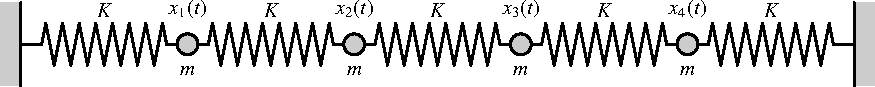
\includegraphics[width=\hsize]{images/e-1}
\end{center}
\caption{Federkette}
\index{Federkette}
\end{figure}
Wir betrachten $n$ gleiche Massen $m$, welche in einer Kette mit gleich
starken Federn miteinander verbunden sind.
Am Ende sind die Massen
ebenfalls mit einer Feder verankert.
Die Massen sollen sich nur entlang der Achse der Federkette bewegen können.
Die Variablen $x_i(t)$ sind Funktionen, die die Auslenkung der Masse mit
Nummer $i$ zur Zeit $t$ aus der Ruhelage beschreibt.
Die Bewegungsgleichung sagt,
dass die zweite Ableitung der Position die von den Federn bewirkte Kraft
ist.
Die Federkraft ist proportional zum Auslenkungsunterschied
$x_{i+1}(t)-x_i(t)$ für die ``rechte'' Feder, bzw.~
$x_{i}(t)-x_{i-1}(t)$ für die ``linke'' Feder.
Die Kraft ist also
\begin{align*}
m\frac{d^2x_i(t)}{dt^2}
&=K((x_{i+1}(t)-x_i(t))-(x_i(t)-x_{i-1}(t)))\\
&=K(x_{i+1}(t)-2x_i(t)+x_{i-1}(t))
\end{align*}
Aus der Erfahrung wissen wir, dass so eine Federkette schwingt, wir nehmen also
an, dass wir eine Lösung in der Form $x_i(t)=x_i(0)\sin\omega t$ finden
können.
Setzen wir dies ein, erhalten wir die Gleichungen
\[
-m\omega^2\sin\omega t x_i(0)=K(x_{i+1}(0)-2x_i(0)+x_{i-1}(0))\sin\omega t.
\]
Da diese Gleichung für alle Zeitpunkte gelten muss, gilt sie auch für
Zeitpunkte, an denen $\sin\omega t\ne 0$, so dass man durch $\sin\omega t$
teilen kann:
\[
-m\omega^2 x_i(0)=K(x_{i+1}(0)-2x_i(0)+x_{i-1}(0)).
\]
Für die Endpunkte der Kette gelten einfachere Formeln.
Auf die Masse $1$
wirkt die Feder links mit der Kraft $-Kx_1(t)$, die Feder rechts übt die
Kraft $K(x_2(t)-x_1(t))$ aus, so dass die Bewegungsgleichung hier zu
\[
-m\ddot x_1(t)=K(-2x_1(t)+x_2(t)),
\]
die Gleichung für die Anfangswerte wird
\[
\omega^2 x_1(0)=-\frac{K}{m}(-2x_1(0)+x_2(0)),
\]
und analog am anderen Ende des Intervalls.

Diese Gleichung soll jetzt auch noch in Matrizenform geschrieben werden.
Die Anfangswerte $x_i(0)$ fassen wir in einen Vektor $x(0)$ zusammen.
Die rechte Seite der Gleichung wird durch die Wirkung der $n\times n$-Matrix
\[
\Delta=
-\frac{K}{m}
\begin{pmatrix}
-2&1&0&0&0&\dots&&&0\\
1&-2&1&0&0&&&&\\
0&1&-2&1&0&&&&\\
0&0&1&-2&1&&&&\\
\vdots&&&&&\ddots&&\\
 &&&&&&-2&1&0\\
 &&&&&&1&-2&1\\
0&&&&&&0&1&-2
\end{pmatrix}
\]
beschrieben.

Unbekannt ist jetzt offenbar, welche Werte $\omega$ überhaupt eine nicht-%
triviale Lösung ermöglichen, also einen Vektor $x$ mit der Eigenschaft
\[
\Delta x=\lambda x
\]
mit $\lambda=\omega^2$.
Wenn wir die zulässigen $\lambda$ bestimmen können,
für die sich eine Lösung $x$ finden lässt, dann kennen wir offenbar auch
die Eigenfrequenzen, mit denen die Federkette schwingen kann.

\subsubsection{Zwei Massen}
Für nur zwei Massen wird die Matrix $\Delta$ zu
\[
\Delta=\begin{pmatrix}
2&-1\\
-1&2
\end{pmatrix}.
\]
Um die Werte $\lambda$ zu finden, für die $\Delta-\lambda E$ singulär
wird, können wir das Determinanten-Kriterium verwenden:
\begin{align*}
\left|\;\begin{matrix}
2-\lambda&-1\\-1&2-\lambda
\end{matrix}\;\right|
&=(2-\lambda)^2-1=\lambda^2 -4\lambda+3=0.
\\
\Rightarrow\qquad
\lambda_{\pm}&=2\pm\sqrt{2^2-3}=\begin{cases}3\\1\end{cases}
\end{align*}
Die Eigenvektoren sind Lösungen des homogenen Gleichungssystems mit
Koeffizientenmatrix $\Delta-\lambda E$.
Einen Vektor im Nullraum
von
\begin{align*}
\lambda&=\lambda_-=1:&
(\Delta -1\cdot E)v_-&=
\begin{pmatrix}
1&-1\\-1&1
\end{pmatrix}v_-=0
&
v_-&=\begin{pmatrix}1\\1\end{pmatrix}
\\
\lambda&=\lambda_+=3:&
(\Delta -3\cdot E)v_+&=
\begin{pmatrix}
-1&-1\\-1&-1
\end{pmatrix}v_+=0
&
v_+&=\begin{pmatrix}1\\-1\end{pmatrix}
\end{align*}
\begin{figure}
\begin{center}
\begin{tabular}{ll}
$\lambda=\lambda_-:$&%
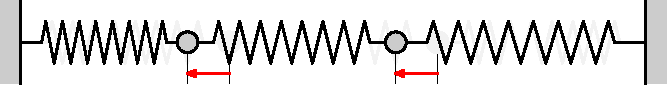
\includegraphics{images/e-4}\\%
&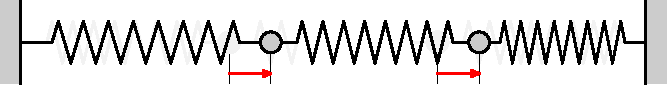
\includegraphics{images/e-5}\\%
\\
$\lambda=\lambda_+:$&%
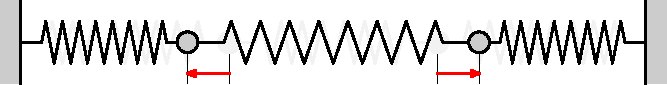
\includegraphics{images/e-2}\\%
&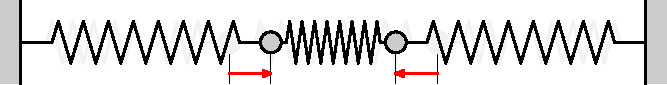
\includegraphics{images/e-3}%
\end{tabular}
\end{center}
\caption{Schwingungsmodi einer Federkette mit zwei Massen ( $n=2$)\label{n2modi}}
\end{figure}%
Es gibt also zwei Schwingungsmodi, in
Abbildung~\ref{n2modi} werden jeweils die beiden Extremlagen 
gezeigt.
Bei der langsamen Schwingung mit Kreisfrequenz
$\omega_-=\sqrt{\lambda_-}=1$ bewegen sich die Massen gleichphasig,
was auch angezeigt wird durch die gleichen Vorzeichen
der Komponenten von $v_-$.
Bei der schnellen Schwingung mit Kreisfrequenz
$\omega_+=\sqrt{\lambda_+}=\sqrt{3}\simeq 1.732$ bewegen sich die 
beiden Massen gegenphasig, ausgedrückt auch durch
die verschiedenen Vorzeichen der Komponenten von $v_+$.

\subsubsection{Drei Massen}
Auch für drei Massen lässt sich das Eigenwertproblem noch
``von Hand'' lösen.
Wir verwenden wieder das Determinanten-Kriterium
\begin{align*}
\det(\Delta -\lambda E)&=\left|\;
\begin{matrix}
2-\lambda&-1&0\\
-1&2-\lambda&-1\\
0&-1&2-\lambda
\end{matrix}
\;\right|
=-\lambda^3+6\lambda^2-10\lambda+4=-(\lambda-2)(\lambda^2-4\lambda+2)
\\
\Rightarrow\qquad
\lambda_1&=2\\
\lambda_{2,3}&=2\pm\sqrt{2^2-2}=2\pm\sqrt{2}
\end{align*}
Für die Eigenvektoren finden wir
\begin{align*}
\lambda&=\lambda_1=2:
&
(\Delta - 2\cdot E)v_1&=\begin{pmatrix}
0&-1&0\\
-1&0&-1\\
0&-1&0\end{pmatrix}v_1
=0&v_1&=\begin{pmatrix}1\\0\\-1\end{pmatrix}
\\
\lambda&=\lambda_2=2+\sqrt{2}:
&
(\Delta -(2+\sqrt{2})E)v_2&=\begin{pmatrix}
-\sqrt{2}&-1&0\\
-1&-\sqrt{2}&-1\\
0&-1&-\sqrt{2}
\end{pmatrix}v_2=0&
v_2&=\begin{pmatrix}
1\\-\sqrt{2}\\1
\end{pmatrix}
\\
\lambda&=\lambda_3=2-\sqrt{2}:
&
(\Delta -(2-\sqrt{2})E)v_2&=\begin{pmatrix}
\sqrt{2}&-1&0\\
-1&\sqrt{2}&-1\\
0&-1&\sqrt{2}
\end{pmatrix}v_2=0&
v_2&=\begin{pmatrix}
1\\\sqrt{2}\\1
\end{pmatrix}
\\
\end{align*}
\begin{figure}
\begin{center}
\begin{tabular}{l}
geringste Eigenfrequenz: $\lambda=\lambda_3$:\\
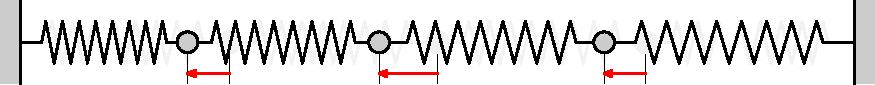
\includegraphics[width=\hsize]{images/e-8}\\
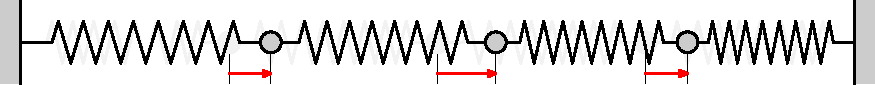
\includegraphics[width=\hsize]{images/e-9}\\
\\
mittlere Eigenfrequenz: $\lambda=\lambda_1$:\\
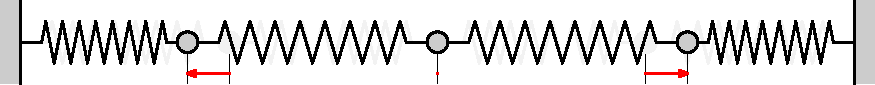
\includegraphics[width=\hsize]{images/e-6}\\
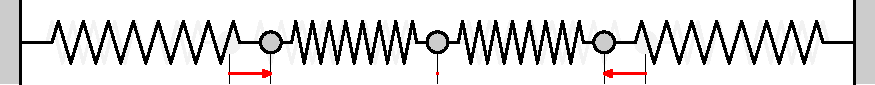
\includegraphics[width=\hsize]{images/e-7}\\
\\
höchste Eigenfrequenz: $\lambda=\lambda_2$:\\
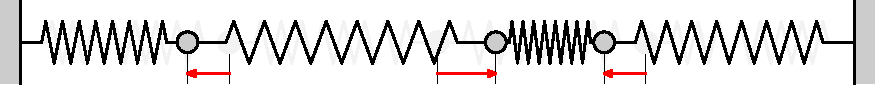
\includegraphics[width=\hsize]{images/e-10}\\
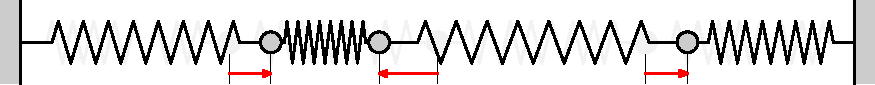
\includegraphics[width=\hsize]{images/e-11}
\end{tabular}
\end{center}
\caption{Schwingungsmodi einer Kette mit drei Massen ($n=3$)\label{n3modi}}
\end{figure}%
Diesmal gibt es drei Schwingungsmodi, von denen in Abbildung~\ref{n3modi}
wieder jeweils die Extremlagen dargestellt sind.
Zur geringsten Frequenz
$\omega_3=\sqrt{\mathstrut\lambda_3}=\sqrt{2-\sqrt{2\mathstrut}}\simeq 0.7654$
gehört eine Schwingung, bei der alle drei Massen in Phase
hin- und herschwingen, wobei die mittlere Masse eine 41\% 
grössere Amplitude hat (Abbildung~\ref{n3modi} unten).
Zur höchsten Frequenz
$\omega_2=\sqrt{\lambda_2}=\sqrt{2+\sqrt{2}}\simeq 1.848$
gehört eine Schwingung, bei der die äusseren Massen in Phase sind,
aber gegenphasig zur mittleren Massen schwingen, die wieder etwa
41\% grössere Amplitude hat (Abbildung~\ref{n3modi} Mitte).
Die mittlere Frequenz $\omega_1=\sqrt{\lambda_1}=\sqrt{2}\simeq 1.414$
gehört zu einer Schwingung, bei der die mittlere Masse stehenbleibt,
während die äusseren beiden Massen gegenphasig schwingen (Abbildung~\ref{n3modi} oben).

\subsubsection{Numerische Resultate}
Mindestens numerisch kann man jetzt bereits viele bekannte
Schwingungs-Phänomene verstehen.
Schon aus den Beispielen
$n=2$ und $n=3$ ist plausibel, dass bei der langsamsten Schwingung
alle $n$ Massen in Phase schwingen.
Zur höchsten Frequenz wird
dagegen die Schwingung gehören, bei der die geraden untereinander
und die ungeraden Massen untereinander in Phase sind.

\begin{table}
\begin{center}
\begin{tabular}{|>{$}c<{$}|>{$}c<{$}|>{$}c<{$}|}
\hline
i&\omega_i&\omega_i/\omega_1\\
\hline
1& 0.031104& 1.0000\\
2& 0.062200& 1.9998\\
3& 0.093281& 2.9990\\
4& 0.124339& 3.9976\\
5& 0.155368& 4.9952\\
6& 0.186359& 5.9915\\
7& 0.217304& 6.9865\\
\hline
\end{tabular}
\end{center}
\caption{Eigenfrequenzen einer Federkette mit $n=100$ Massen.
\label{frequenzen-federkette}}
\end{table}

Bestimmen wir die Eigenfrequenzen für $n=100$ numerisch, finden wir
die Frequenzen in Tabelle~\ref{frequenzen-federkette}.
Es fällt auf, dass
in guter Näherung die höheren Eigenfrequenzen ganzzahlige Vielfache
der Grundfrequenz sind.

\begin{figure}
\begin{center}
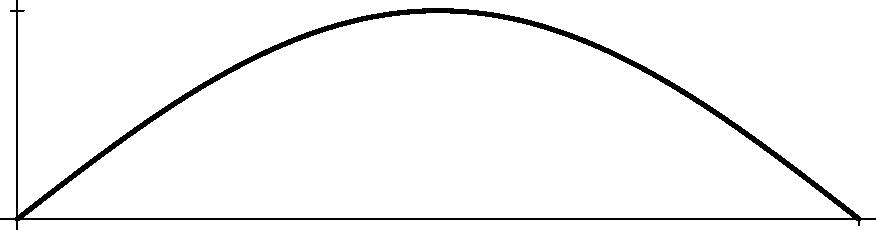
\includegraphics[width=\hsize]{images/e-12}\\
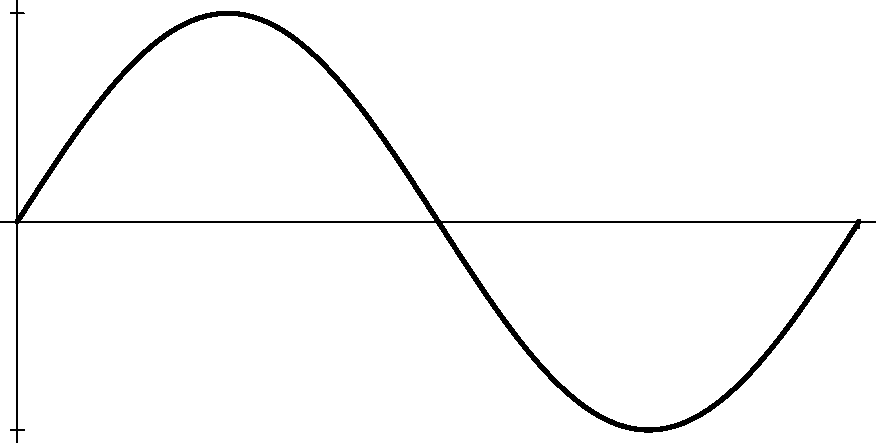
\includegraphics[width=\hsize]{images/e-13}\\
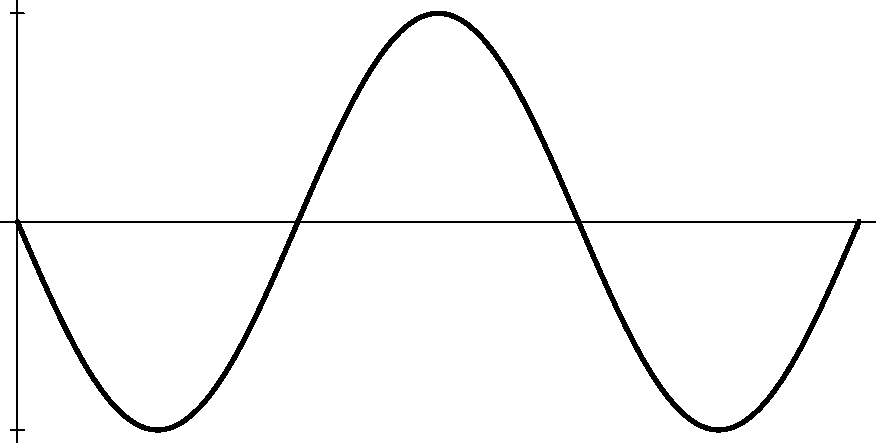
\includegraphics[width=\hsize]{images/e-14}
\end{center}
\caption{Die ersten drei Eigenvektoren einer Federkette mit $n=100$
Massen\label{eigenvektoren-n100}}
\end{figure}
In Abbildung \ref{eigenvektoren-n100} sind die Komponenten der drei
Eigenvektoren mit der geringsten Frequenz dargestellt.
Die Ähnlichkeit mit den Sinusfunktionen lässt sich dadurch erklären,
dass die Federkette die diskrete Variante eines kontinuierlichen
Problems ist, nämlich der Schwingung einer Saite, deren Lösungen
tatsächlich die trigonometrischen Funktionen sind.

\subsection{Fibonacci-Zahlen}
\index{Fibonacci-Folge}
In der Folge der Fibonacci-Zahlen
\[
0,1,1,2,3,5,8,13,21,34,55,89,144,\dots
\]
entsteht das nächste Element als Summe der beiden vorangegangenen
Elemente.
Die Folge ist offenbar festgelegt, wenn man die zwei ersten
Werte $0$ und $1$ festlegt.
Durch Wahl eines anderen Paares von Startzahlen
erhält man eine alternative Fibonacci-Folge.
Die Fibonacci-Zahlen
erfüllen die Gleichung 
\[
x_{n+1}=x_n+x_{n-1},
\]
die wir
auch 
\begin{equation}
x_{n+1}-x_n-x_{n-1}=0
\end{equation}
schreiben können.
Eine solche Gleichung heisst eine Differenzengleichung.

\begin{figure}
\begin{center}
\begin{tabular}{cc}
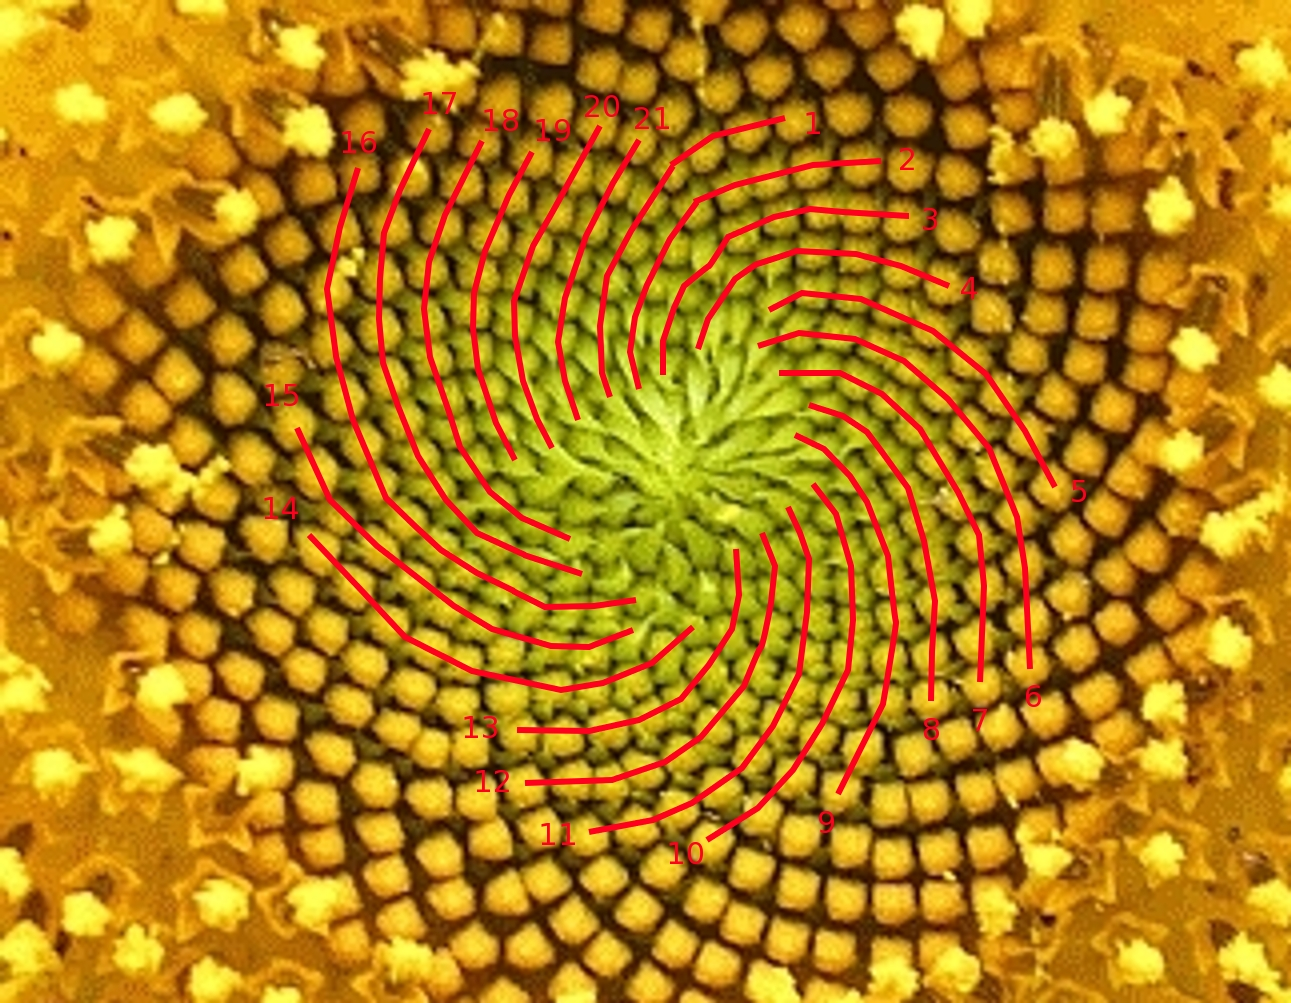
\includegraphics[width=0.47\hsize]{graphics/helianthus-fibonacci2.jpg}&%
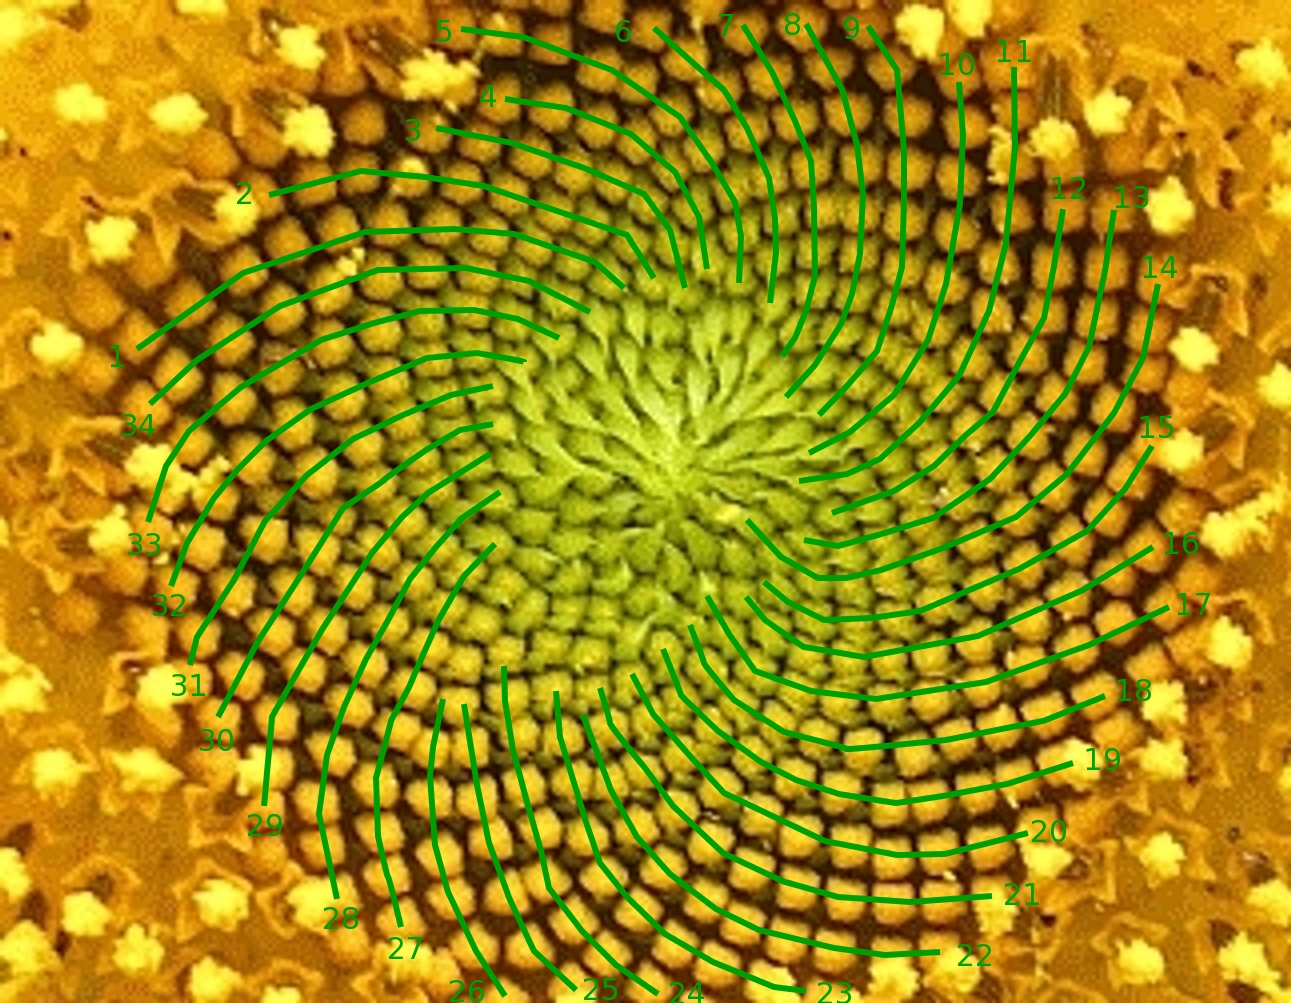
\includegraphics[width=0.47\hsize]{graphics/helianthus-fibonacci3.jpg}\\%
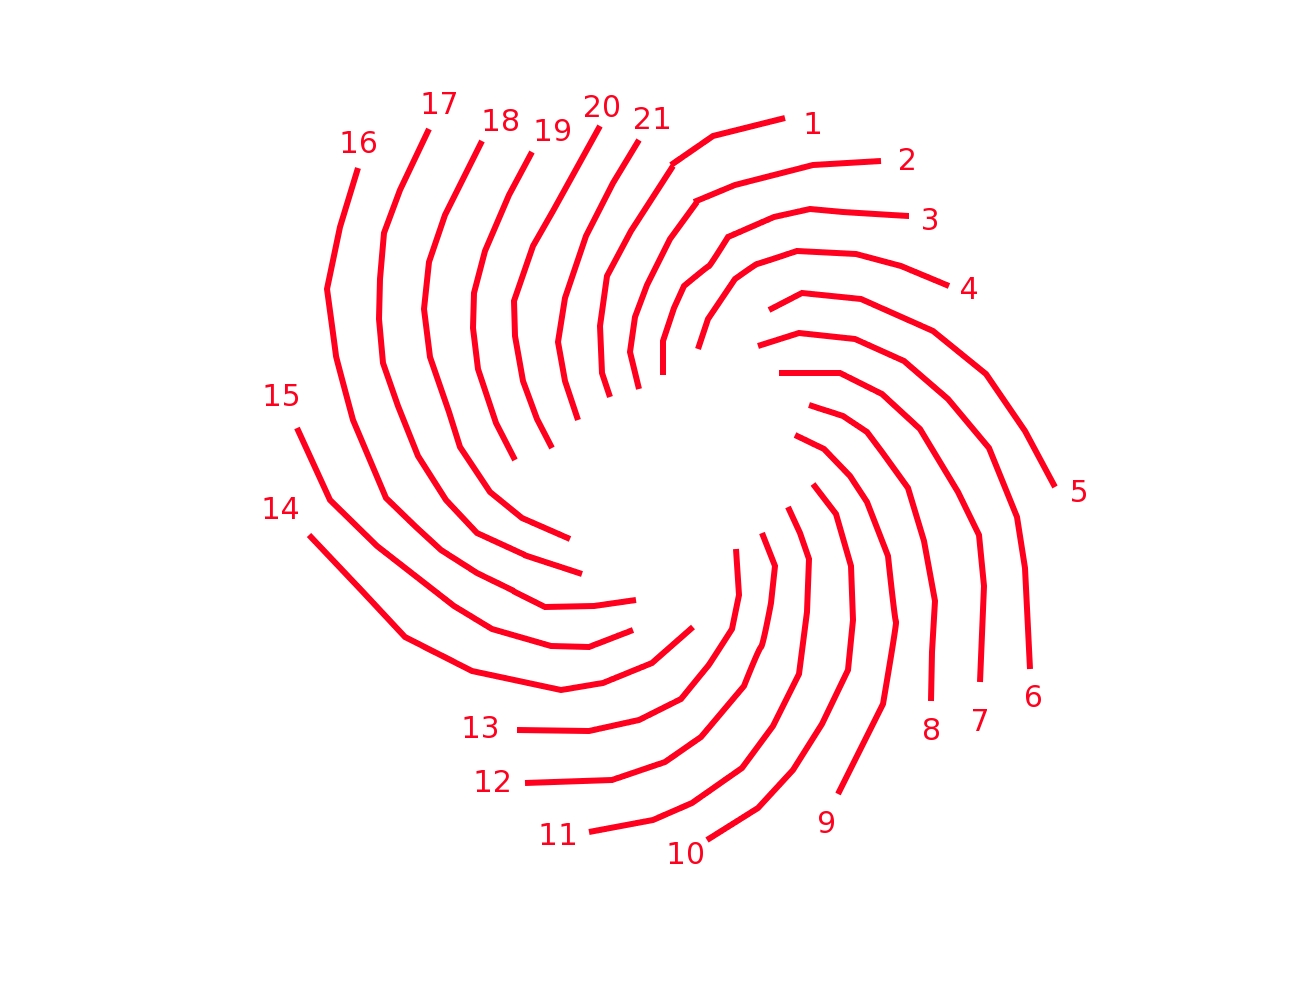
\includegraphics[width=0.47\hsize]{graphics/helianthus-fibonacci5.jpg}&%
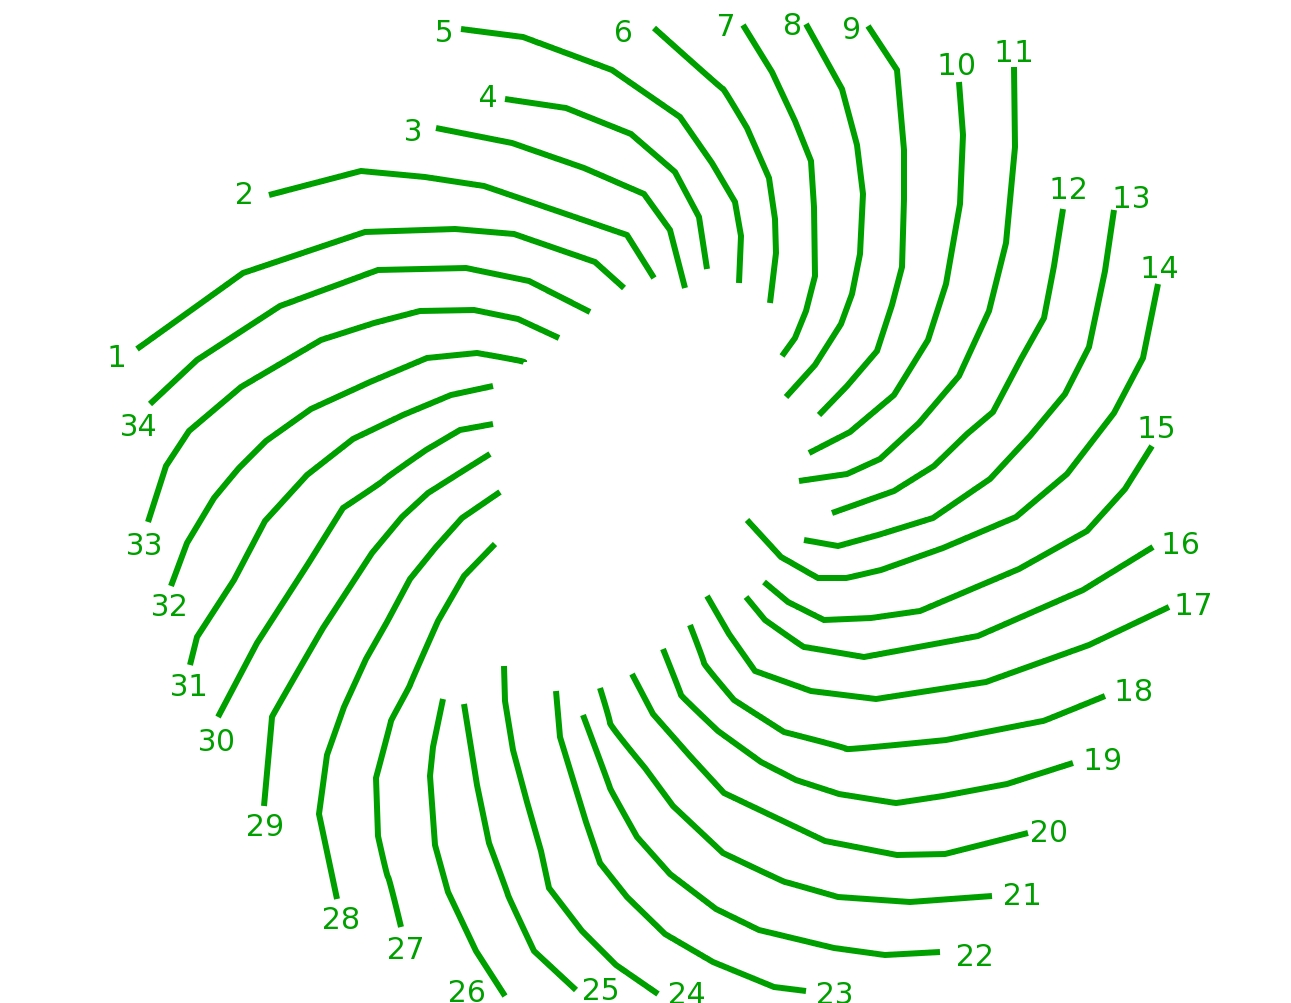
\includegraphics[width=0.47\hsize]{graphics/helianthus-fibonacci4.jpg}
\end{tabular}
\end{center}
\caption{Die Anzahl der Spiralen in den Blütenständen von Sonnenblumen
sind aufeinanderfolgende Fibonacci-Zahlen, hier $21$ (rot) und $34$ (grün).
\label{helianthus}}
\end{figure}

Die Fibonacci-Zahlen kommen erstaunlich oft vor:
\begin{itemize}
\index{Sonnenblume}
\index{Tannzapfen}
\index{Ananas}
\index{Romanesco-Broccoli}
\index{goldener Schnitt}
\index{Lateralus}
\item In den Blütenständen von Sonnenblumen kann man jeweils zwei
Scharen von Spiralen erkennen, auf denen die Sonnenblumenkerne angeordnet sind.
Die Anzahlen der Spiralen in jeder Schar sind jeweils zwei aufeinanderfolgende
Fibonacci-Zahlen (Abbildung~\ref{helianthus}).
\item Auch in Tannenzapfen, auf einer Ananas oder auf Romanesco-Broccoli
kann man diese Spiralen erkennen.
\item Das Verhältnis aufeinanderfolgender Fibonacci-Zahlen strebt gegen
$\frac{1+\sqrt{5}}2$, dem Verhältnis des goldenen Schnittes, dem schon die
Griechen besondere ästhetische Qualitäten nachsagten.
\item Im Song `Lateralus' der Gruppe Tool ist die Anzahl der Silben
in jedem Textblock eine Fibonacci-Zahl, und auch der Rhythmus basiert
auf den Fibonacci-Zahlen.
\end{itemize}

\subsubsection{Rekursionsgleichung als Matrizengleichung}
\index{Rekursionsgleichung}
Um die Fibonacci-Zahlen zu berechnen, muss man sich nur jeweils die letzten zwei
Zahlen merken, wir schreiben diese in eine Spaltenvektor
\[
\begin{pmatrix}x_n\\x_{n-1}\end{pmatrix}.
\]
Beim Übergang zur Fibonacci-Zahl $x_{n+1}$ muss man sich auch $x_n$ merken,
man muss also den neuen Spaltenvektor berechnen:
\begin{equation}
\begin{pmatrix}x_{n+1}\\x_n\end{pmatrix}
=
\begin{pmatrix}x_n+x_{n-1}\\x_n\end{pmatrix}
=
\begin{pmatrix}
1&1\\
1&0
\end{pmatrix}
\begin{pmatrix}x_n\\x_{n-1}\end{pmatrix}
=
A
\begin{pmatrix}x_n\\x_{n-1}\end{pmatrix}.
\label{fibonaccirekursion}
\end{equation}
\subsubsection{Lösung als Eigenwertproblem}
Natürlich ist es etwas umständlich, zum Beispiel die 1291-ste Fibonacci-Zahl
zu berechnen, da wäre eine Formel $f(n)$ sehr praktisch, in der man einfach
die Zahl 1291 einsetzen könnte.
Die Fibonacci-Zahlen nehmen sehr schnell zu, 
wir versuchen die Lösung in der Form
\[
f(n)=a\lambda^n
\]
zu finden. Eingesetzt in (\ref{fibonaccirekursion}) ergibt sich
\[
\begin{pmatrix}a\lambda^{n+1}\\a\lambda^n\end{pmatrix}
=A\begin{pmatrix}a\lambda^n\\a\lambda^{n-1}\end{pmatrix}.
\]
Der Vektor auf der linken Seite ist das $\lambda$-fache des Vektors
auf der rechten Seite, wenn es also überhaupt eine Lösung in der
Form $f(n)=a\lambda^n$ gibt, dann gibt es auch einen Vektor $y$, der
die Gleichung
\begin{equation}
Ay=\lambda y, \qquad y=\begin{pmatrix}
a\lambda^n\\a\lambda^{n-1}
\end{pmatrix}
\end{equation}
erfüllt. In diesem Gleichungssystem kommen die Unbekannten auch auf
der rechten Seite vor, die Standard-Form ist daher
\[
Ay-\lambda y=(A-\lambda I)y=0.
\]
Wir müssen also herausfinden, für welche Werte von $\lambda$ dieses
Gleichungssystem überhaupt eine nichttriviale Lösung (und damit unendlich
viele Lösungen) hat.
Dies geschieht genau dann, wenn die Determinante der Matrix
\[
A-\lambda I=\begin{pmatrix}1-\lambda&1\\1&-\lambda\end{pmatrix}
\]
verschwindet.
Berechnung der Determinante ergibt die quadratische Gleichung
\[
\det
\begin{pmatrix}1-\lambda&1\\1&-\lambda\end{pmatrix}
=(1-\lambda)(-\lambda)-1=\lambda^2-\lambda-1=0.
\]
Sie hat die Lösungen
\[
\lambda_{\pm}=\frac12+\pm\sqrt{\frac14+1}=\frac{1\pm\sqrt{5}}2.
\]
Für jeden Wert $\lambda_{\pm}$ gibt es einen nichttrivialen
Lösungsvektor, den man durch Lösen des Gleichungssystems nach
Einsetzen von $\lambda_{\pm}$ erhalten kann.

Setzt man $\lambda_+$ ein, bekommt man die Koeffizientenmatrix
\[
A-\lambda_+I=
\begin{pmatrix}
1-\lambda_+&1\\1&-\lambda_+
\end{pmatrix}
=
\begin{pmatrix}
\frac{1-\sqrt{5}}2&1\\1&-\frac{1+\sqrt{5}}2
\end{pmatrix}
\]
Wir wissen bereits, dass das Gleichungssystem $(A-\lambda_+I)y=0$
eine nichttriviale Lösung hat, zum Beispiel
\[
y_+=\begin{pmatrix}
\frac{1+\sqrt{5}}2\\1
\end{pmatrix}
=\begin{pmatrix}
\lambda_+\\1
\end{pmatrix}
\]
Analog hat man für $\lambda_-$ die Matrix
\[
A-\lambda_-I=
\begin{pmatrix}
\frac{1+\sqrt{5}}2&1\\
1&-\frac{1-\sqrt{5}}2
\end{pmatrix}
\]
und eine nichttriviale Lösung 
\[
y_-=\begin{pmatrix}
\frac{1-\sqrt{5}}2\\
1
\end{pmatrix}=
\begin{pmatrix}
\lambda_-\\1
\end{pmatrix}
\]
\subsubsection{Anfangswerte}
Wir haben inzwischen die Folgen
\[
\begin{matrix}
1&\lambda_+&\lambda_+^2&\lambda_+^3&\lambda_+^4&\dots\\
1&\lambda_-&\lambda_-^2&\lambda_-^3&\lambda_-^4&\dots
\end{matrix}
\]
gefunden, die beide Lösungen des Rekursionsgleichung sind, die Summe
zweier Folgenglieder ergibt das nächste Glied.
Diese Eigenschaft bleibt auch erhalten, wenn wir zwei beliebige
Vielfache dieser Folgen addieren.
Die Folge
\[
\begin{matrix}
A+B,
&A\lambda_++B\lambda_-,
&A\lambda_+^2+B\lambda_-^2,
&A\lambda_+^3+B\lambda_-^3,
&\dots
&A\lambda_+^n+B\lambda_-^n,
&\dots
\end{matrix}
\]
ist auch eine Lösung der Rekursionsgleichung.
Tatsächlich können
wir die Lösung
$x_n=A\lambda_+^n + B\lambda_-^n$
in die Rekursionsgleichung einsetzen:
\begin{align*}
x_{n+1}-x_n-x_{n-1}
&=A\lambda_+^{n+1} + B\lambda_-^{n+1}
-x_n=A\lambda_+^n - B\lambda_-^n
-x_{n-1}=A\lambda_+^n - B\lambda_-^{n-1}
\\
&=
A(\lambda_+^{n+1}-\lambda_+^n-\lambda_+^{n-1})
+
B(\lambda_-^{n+1}-\lambda_-^n-\lambda_-^{n-1})
\\
&=0
\end{align*}
Die Klammerausdrücke verschwinden, weil $\lambda_+^n$ und $\lambda_-^n$
für sich bereits Lösungen der Rekursionsgleichung sind.

Wir möchten jetzt eine Folge konstruieren, die mit bestimmten Werten
$0$ und $1$ beginnt, dazu müssen wir die Koeffizienten $A$ und $B$
bestimmen:
\[
\begin{matrix}
A\phantom{\lambda_+}&+&B\phantom{\lambda_-}&=&0
\\
A\lambda_+&+&B\lambda_-&=&1
\end{matrix}
\]
Es ist also ein Gleichungssystem mit Matrix
\[
\begin{pmatrix}
1&1\\\lambda_+&\lambda_-
\end{pmatrix}
\]
und den gewünschten Anfangswerten als rechten Seiten zu lösen.
In diesem speziellen Fall ist das Determinanten-Verfahren zweckmässig:
\begin{align*}
A&=\frac{
\left|
\begin{matrix}
0&1\\1&\lambda_-
\end{matrix}
\right|
}{
\left|
\begin{matrix}
1&1\\\lambda_+&\lambda_-
\end{matrix}
\right|
}
=
\frac{-1}{\lambda_--\lambda_+}=-\frac1{-\sqrt{5}}=\frac1{\sqrt{5}}
\\
B&=\frac{
\left|
\begin{matrix}
1&0\\\lambda_+&1
\end{matrix}
\right|
}{
\left|
\begin{matrix}
1&1\\\lambda_+&\lambda_-
\end{matrix}
\right|
}
=
\frac{1}{\lambda_--\lambda_+}=\frac1{-\sqrt{5}}=-\frac1{\sqrt{5}}
\end{align*}
Somit ist die Folge
\begin{equation}
x_n=\frac1{\sqrt{5}}\left(\frac{1+\sqrt{5}}{2}\right)^n
-\frac1{\sqrt{5}}\left(\frac{1-\sqrt{5}}{2}\right)^n
\label{fibonacci}
\end{equation}
die gesuchte geschlossene Formel für die Fibonacci-Zahlen.
Es ist auf den ersten Blick überraschend, dass die Formel
(\ref{fibonacci}) für jeden Wert von $n$ einen natürliche
Zahl ergibt, obwohl jeder einzelne Summand irrational ist.

Man kann aus (\ref{fibonacci}) auch andere Eigenschaften der
Fibonacci-Zahlen ablesen.
Zum Beispiel ist der Quotient zweier aufeinanderfolgender Fibonacci-Zahlen
\begin{align*}
\frac{x_{n+1}}{x_n}
&=
\frac{A\lambda_+^{n+1}+B\lambda_-^{n+1}}{A\lambda_+^{n}+B\lambda_-^{n}}
=
\lambda_+\frac{1+\displaystyle\frac{B\lambda_-^{n+1}}{A\lambda_+^{n+1}}}{1+\displaystyle\frac{B\lambda_-^n}{A\lambda_+^n}}
=
\lambda_+\frac{1-q^{n+1}}{1-q^n},
\end{align*}
wobei $q=\lambda_+/\lambda_-$.
Da $q<1$ ist, werden die Potenzen $q^n$ für grosse $n$ beliebig klein,
und damit auch
\[
\lim_{n\to\infty}\frac{x_{n+1}}{x_n}=\lambda_+,
\]
der Quotient aufeinanderfolgender Fibonacci-Zahlen strebt also gegen
$\lambda_+$.

\subsubsection{Verallgemeinerung}
Das eben dargestellte Verfahren zur Lösung einer endlichen 
Differenzengleichung lässt sich verallgemeinern.
Eine Differenzengleichung der Form
\[
x_{n+1}=a_kx_n+a_{k-1}x_{n-1}+\dots+a_1x_{n-k+1}+a_0x_{n-k}
\]
kann in vektorieller Form als
\[
\begin{pmatrix}
x_{n-k+1}\\
x_{n-k+2}\\
\vdots\\
x_{n}\\
x_{n+1}
\end{pmatrix}
=
\begin{pmatrix}
0&1&0&\dots&0\\
0&0&1&\dots&0\\
\vdots&\vdots&\vdots&\ddots&\vdots\\
0&0&0&\dots&1\\
a_0&a_1&a_2&\dots&a_k
\end{pmatrix}
\begin{pmatrix}
x_{n-k}\\
x_{n-k+1}\\
\vdots\\
x_{n-1}\\
x_n
\end{pmatrix}
\]
geschrieben werden, wir bezeichnen die $k\times k$-Matrix mit $A$.
Mit einem Ansatz der Form $x_n=\lambda^n$ und
\[
x=
\begin{pmatrix}
\lambda^{n-k}\\
\vdots\\
\lambda^n
\end{pmatrix}
\]
wird daraus ein
Eigenwert-Problem
\[
\begin{pmatrix}
\lambda_{n-k+1}\\
\vdots\\
\lambda^{n+1}
\end{pmatrix}
=
\lambda x
=A
\begin{pmatrix}
\lambda^{n-k}\\
\vdots\\
\lambda^n
\end{pmatrix}
=Ax
\]
Im allgemeinen wird es $k$ verschiedene Werte $\lambda_1,\dots\lambda_k$ geben,
für die dieses Gleichungssystem eine nichttriviale Lösung hat.
Eine Linearkombination der Lösungen $\lambda_i^n$ ist wiederum eine
Lösung der Differenzengleichung.
Sogar die Wachstumseigenschaft lässt
sich verallgemeinern: der Quotient aufeinanderfolgender Folgenglieder
einer Lösung strebt gegen den betragsmässig grössten Eigenwert $\lambda_i$
unter den zur Lösung kombinierten $\lambda_i^n$.

